
	\سؤال{مشاهده فراخوانی‌های سیستمی تعریف شده}

در این قسمت با توجه به این‌که ساختار سخت‌افزار ما با سوال فرق دارد، فایل \lr{asm} را به کمک دستور \lr{find} پیدا کردیم:

\begin{code}
	> cd /usr/include/
	
	> find . -name asm
	
	./x86_64-linux-gnu/asm
	
	> cd ./x86_64-linux-gnu/asm/
	
	> cat unistd.h
	
\end{code}

\begin{figure}[h!]
	\centering
	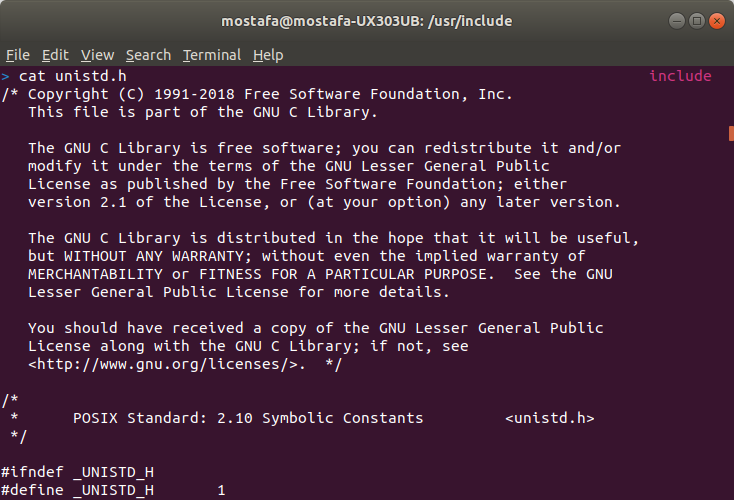
\includegraphics[scale=.4]{img/1.png}
\end{figure}

\سؤال{اجرای یک فراخوانی سیستمی}

\begin{itemize}
	\item 
	دستورات زیر را درون \lr{terminal} اجرا می‌کنیم.
	
	\begin{code}
		> mkdir 2 \&\& cd 2
		
		> sudo nano testsyscall.cpp
		
		
	\end{code}

	\item کد داده شده در سوال را در این قسمت کپی کرده و سپس با استفاده از دستور \lr{\lstinline{ctrl + x}} آن را ذخیره می‌کنیم.
	
	\item به کمک دستورات زیر کد را کامپایل کرده و اجرا می‌کنیم.
	
	\begin{code}
		> sudo gcc -o testsyscall testsyscall.cpp 
		
		> ./testsyscall
	\end{code}

	\item نتیجه‌ی اجرای آن ساخته شدن یک پوشه به نام \lr{testdir} در مسیر   \footnote{directory} فعلی است و در آخر پیام \lr{The result is 0.} را چاپ می‌کند.
	
	\item 
	همان‌طور که در توضیحات فراخوانی سیستمی آمده است، هر فراخوانی سیستم با یک شماره‌ی ثابت شناخته می‌شود. نقش \lr{\lstinline{\_\_NR\_mkdir}} (که به‌طور سراسری \footnote{global} تعریف شده است) در این‌جا این است تا عدد مربوط به این فراخوانی جایگرین آن شود.
	
	\begin{figure}[h!]
		\centering
		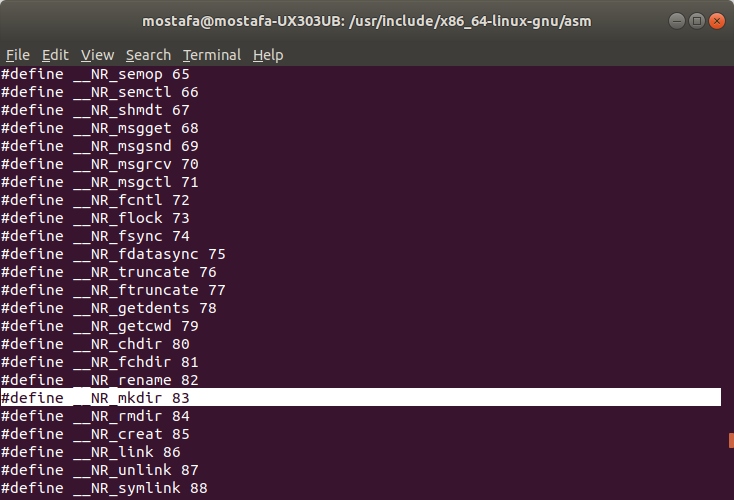
\includegraphics[scale=.4]{img/2.png}
	\end{figure}
	
	\item تابع \lr{\lstinline{syscall()}} یک تابع کوچک است که رابط زبان \lr{assembly} آن دارای شماره و آرگومان‌های مشخص است. تابع پر کاربردی است اگر از آن بدون \lr{wrapper}ها استفاده کنیم، رجسیترهای پردازنده قبل از فراخوانی سیستم ذخیره می‌کند و بعدا آن‌ها را بازگردانی می‌کند. خروجی آن در صورتی که با موفقیت انجام گیرد، «۰» و در غیر این صورت «۱-» خواهد بود.
\end{itemize}

\سؤال{اجرای ساده‌تر فراخوانی‌های سیستمی}
	
	\begin{Verbatim}[tabsize=4]
#include <stdio.h>
#include <unistd.h>
#include <sys/stat.h>
int main() {
	long result;
	result = mkdir("testdir", 0777);
	printf("The result is %ld.\n", result);
	return 0;
}
	\end{Verbatim}
	
	\سؤال{آشنایی با چند فراخوان سیستمی پرکاربرد}
	\begin{itemize}
		
		\item فراخوان سیستمی \lr{access}
			\begin{Verbatim}[tabsize=4]
#include <errno.h>
#include <stdio.h>
#include <unistd.h>

int main(int argc, char *argv[])
{
	int result;
	char *path = argv[1];
	result = access(path, F_OK);
	if (result == 0)
	{
	printf("%s exists\n", path);
	}
	else
	{
	printf("%s doesn't exist\n", path);
	}
	result = access(path, R_OK);
	if (result == 0) {
	printf("read permission is granted\n");
	}
	else {
	printf("read permission isn't granted\n");
	}
	result = access(path, W_OK);
	if (result == 0) {
	printf("write permission is granted\n");
	}
	else {
	printf("write permission isn't granted\n");
	}
	result = access(path, X_OK);
	if (result == 0) {
	printf("execute permission is granted\n");
	}
	else {
	printf("execute permission isn't granted\n");
	}
	return 0;
}
			\end{Verbatim}
			
		\item فراخوان‌های سیستمی \lr{open, close, write}
		\begin{Verbatim}[tabsize=4]
#include <sys/types.h>
#include <sys/stat.h>
#include <fcntl.h>
#include <unistd.h>
#include <string.h>

int main() {
	int open_result;
	int write_result;
	open_result = open("oslab2.txt", O_CREAT | O_WRONLY, 0777);
	write_result = write(open_result, "Mostafa Ghadimi\n", strlen("Mostafa Ghadimi\n"));
	close(open_result);
	return 0;
}

		\end{Verbatim}
		
		\item فراخوان سیستمی \lr{sysinfo}
			\begin{Verbatim}[tabsize=4]

#include <linux/kernel.h>
#include <stdio.h>
#include <sys/sysinfo.h>

int main()
{
	const double megabyte = 1024 * 1024;
	struct sysinfo si;
	sysinfo(&si);
	printf("total RAM: %5.1f MB\n", si.totalram / megabyte);
	printf("free RAM: %5.1f MB\n", si.freeram / megabyte);
	return 0;
}
			\end{Verbatim}
			
		\item فراخوان سیستمی \lr{getrusage}
			\begin{Verbatim}[tabsize=4]
#include <sys/time.h>
#include <sys/resource.h>
#include <stdio.h>

int main() {
	struct rusage ru;
	getrusage(RUSAGE_SELF, &ru);
	printf("maximum resident set size: %ld\n", ru.ru_maxrss);
	printf("integral shared memory size: %ld\n", ru.ru_ixrss);
	printf("integral unshared stack size: %ld\n", ru.ru_isrss);
}
			\end{Verbatim}
	\end{itemize}

\سؤال{اضافه کردن یک فراخوانی سیستمی به سیستم‌عامل}

	\begin{itemize}
		\item با توجه به لینکی که در کلاس داده شد، می‌خواهیم یک فراخوانی سیستمی اضافه کنیم که تعداد \lr{page fault} را نشان دهد.
		\begin{enumerate}
			\item
				 در ابتدا به ۲ فایل \lr{arch/x86/entry/syscalls/syscall_64.tbl} و \lr{arch/x86/entry/syscalls/syscall_32.tbl}، فراخوانی سیستمی دل‌خواه با شماره ۴۳۶ را اضافه می‌کنیم.
				
				\begin{figure}[!h]
					\centering
					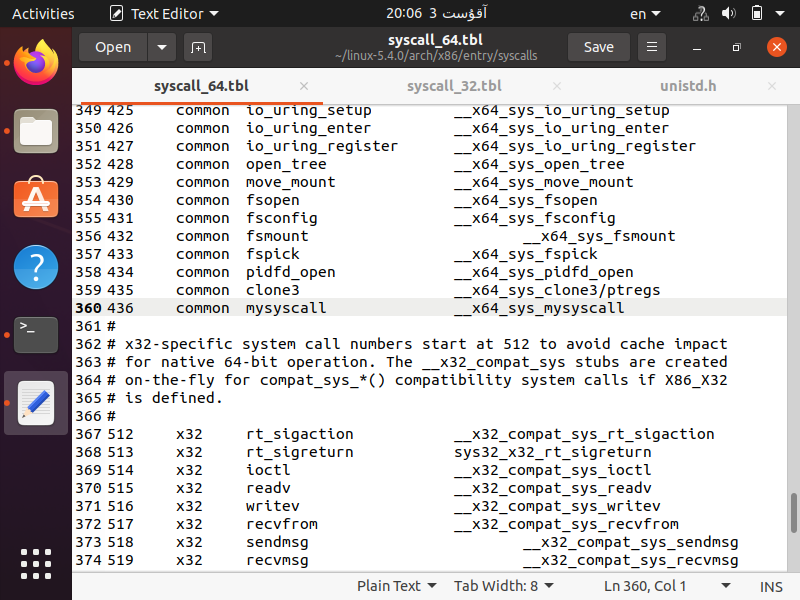
\includegraphics[scale=0.4]{img/pic1.png}
				\end{figure}
				\begin{figure}[!h]
					\centering
					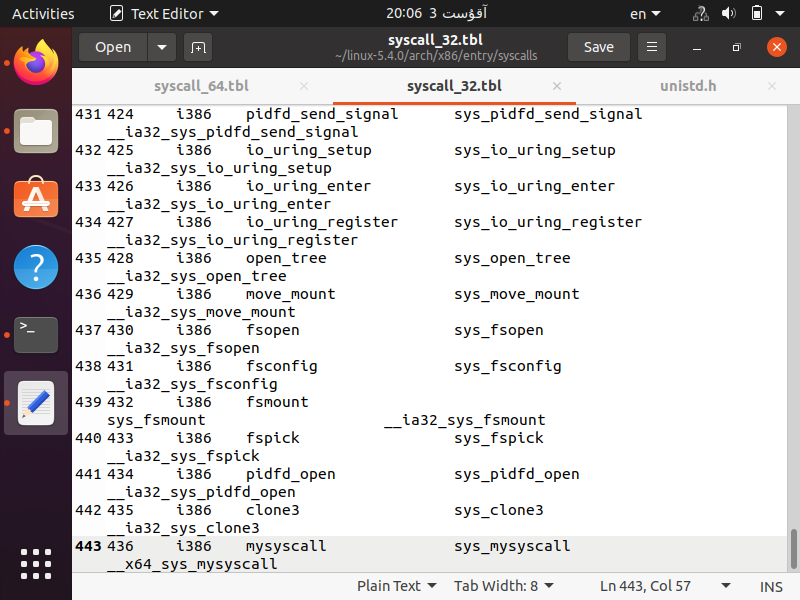
\includegraphics[scale=0.4]{img/pic2.png}
				\end{figure}
			\item 
			 به عنوان \lr{micro} به فایل \lr{include/uapi/asm-generic/unistd.h} آن را اضافه می‌کنیم.
			 \begin{figure}[!h]
			 	\centering
			 	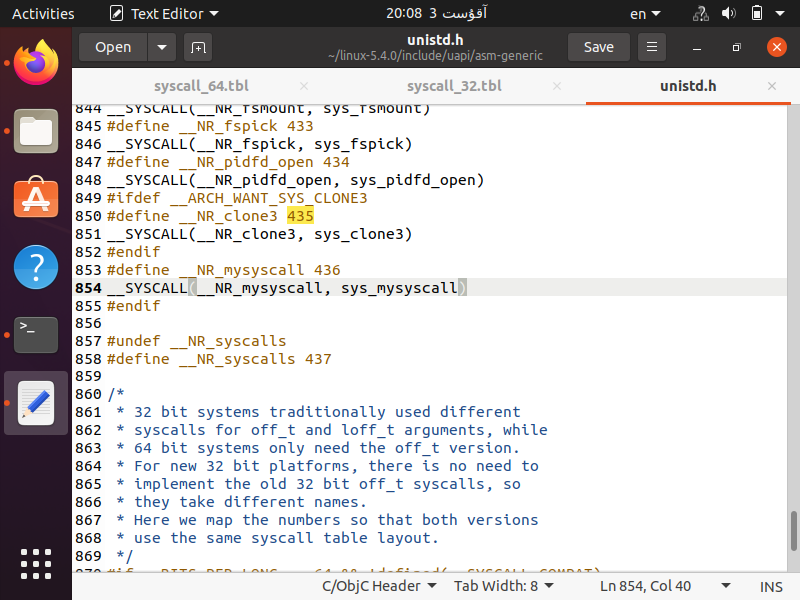
\includegraphics[scale=0.4]{img/pic3.png}
			 \end{figure}
		 \item 	
		 	حال می خواهیم کد خود را در \lr{kernel} اضافه کنیم.
		 	در فایل \lr{include/linux/mm.h}، در انتهای فایل یک متغیر سراسری به نام \lr{pfcount} که نشان‌دهنده تعداد \lr{page fault}ها می‌باشد را اضافه می‌کنیم.
		 	\begin{figure}[!hpbt]
		 		\centering
		 		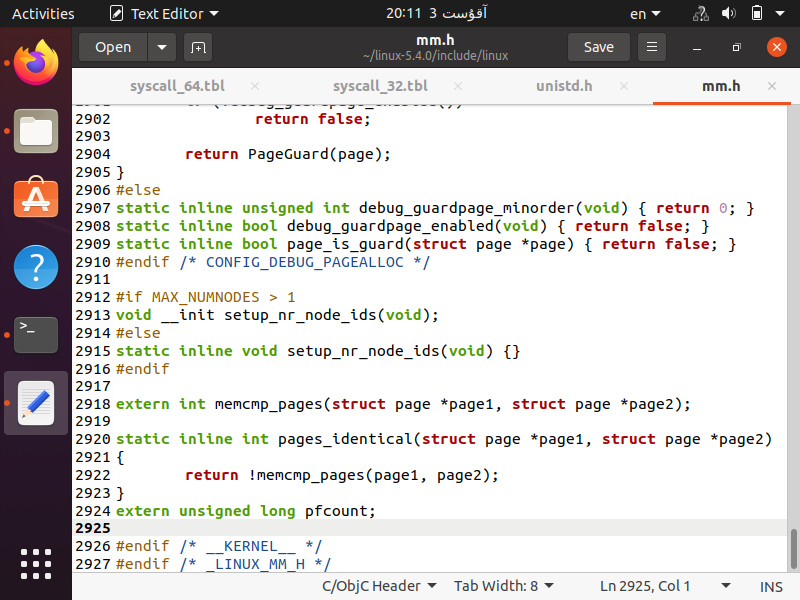
\includegraphics[scale=0.4]{img/pic4.png}
		 	\end{figure}
	 	\item 
	 		 در فایل \lr{include/linux/sched.h}، به \lr{task_struct} (که یک \lr{abstraction} برای پردازه‌های لینوکس می باشد) یک شمارنده \lr{page fault} اضافه می‌کنیم.
	 		\begin{figure}[!hpbt]
	 			\centering
	 			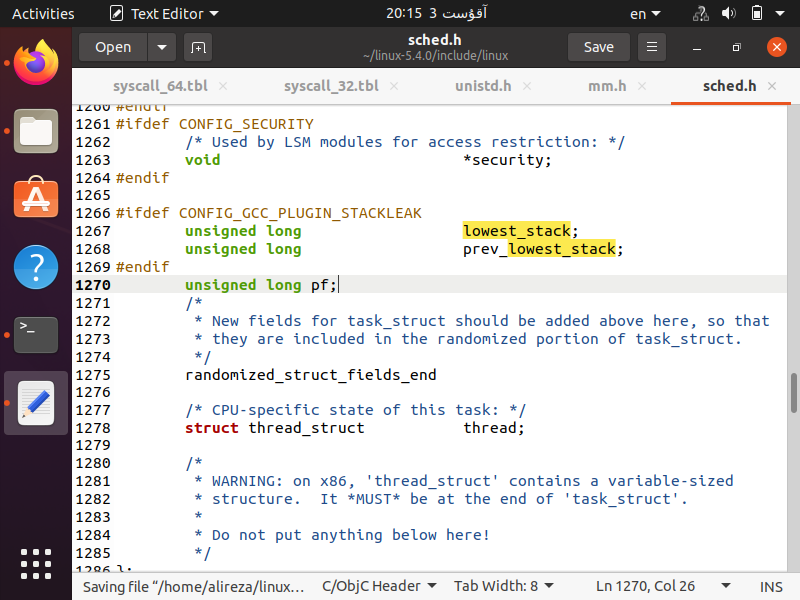
\includegraphics[scale=0.4]{img/pic5.png}
	 		\end{figure}
 			\item 
 				در فایل \lr{kernel/fork.c}، کد \lr{tsk->pf = 0} در جای مشخص اضافه می‌کنیم.
 				\begin{figure}[!hpbt]
 					\centering
 					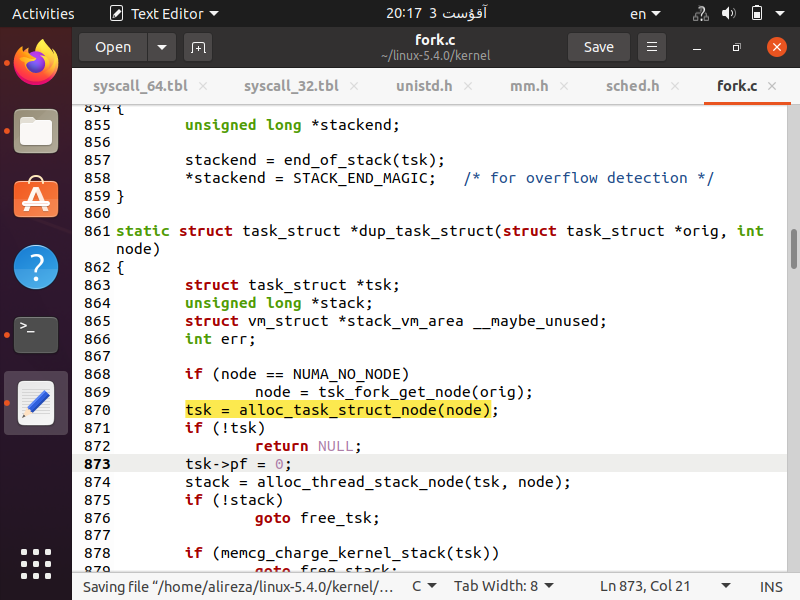
\includegraphics[scale=0.4]{img/pic6.png}
 				\end{figure}
 			\item 
 			حال برای اینکه هر بار \lr{page fault} رخ داد، متغیر خود را افزایش دهیم، در فایل \lr{arch/x86/mm/fault.c} خطوط ۱۵۱۵، ۱۵۲۱ و ۱۵۲۲ را اضافه می‌کنیم.
 			\begin{figure}[!hpbt]
 				\centering
 				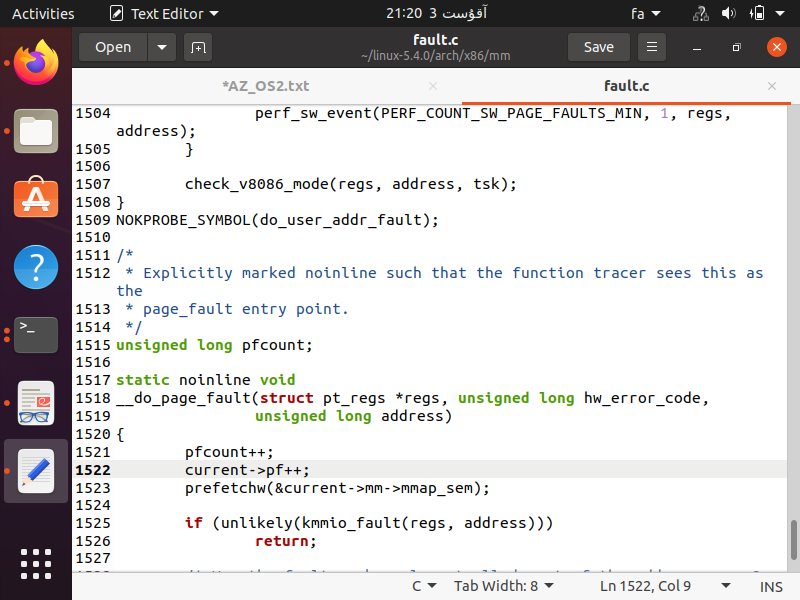
\includegraphics[scale=0.4]{img/pic7.png}
 			\end{figure}
 			
 			\item 
 			برای پیاده سازی تابع \lr{systemcall}، ابتدا کد زیر را به فایل \lr{kernel/sys.c} اضافه می کنیم.
 			\begin{figure}[!hpbt]
 				\centering
 				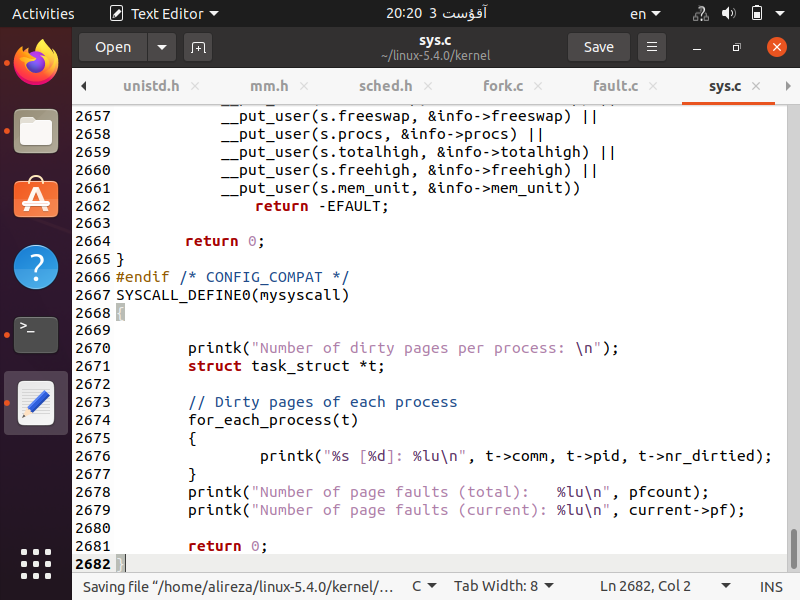
\includegraphics[scale=0.4]{img/pic8.png}
 			\end{figure}
 			\item 
 			 تعریف تابع \lr{systemcall} موردنظر را به فایل \lr{include/linux/syscalls.h} اضافه می‌کنیم.
 			 \begin{figure}[!hpbt]
 			 	\centering
 			 	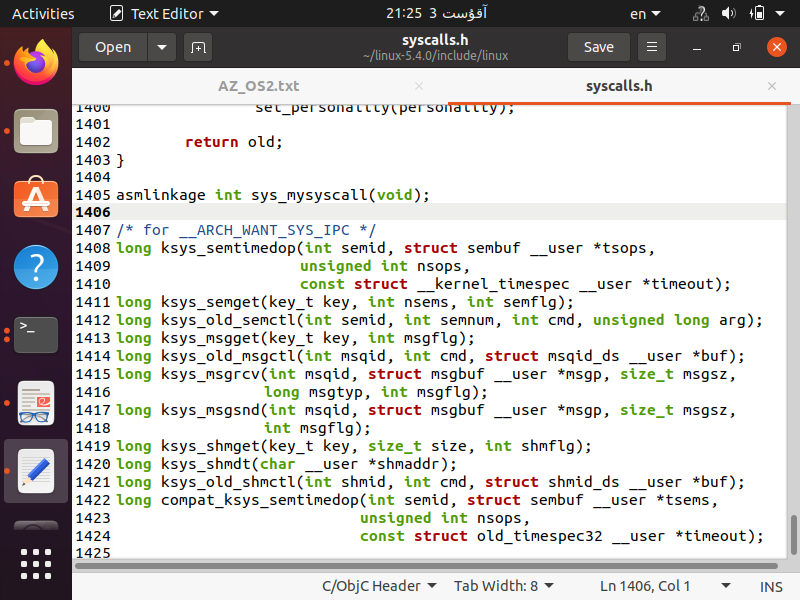
\includegraphics[scale=0.4]{img/pic9.png}
 			 \end{figure}
 			 \item 
 			 
 			 در نهایت برای \lr{compatibility} کد زیر را به فایل \lr{kernel/sys_ni.c} اضافه می‌کنیم.
 			 
 			 \begin{figure}[!hpbt]
 			 	\centering
 			 	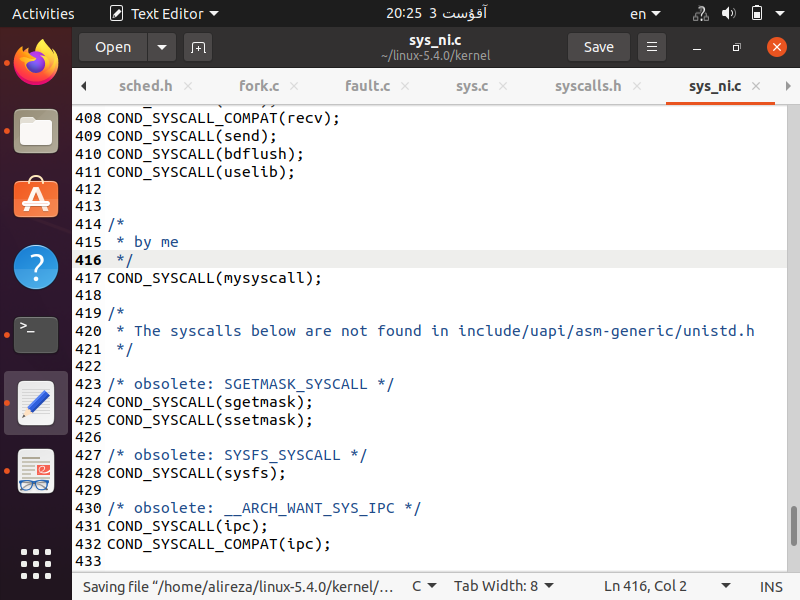
\includegraphics[scale=0.4]{img/pic10.png}
 			 \end{figure}
 		 
 			 \item 
 			 
 			 حال با استفاده از دستور \lr{\& nohup make -j12}، کرنل را کامپایل کرده و با استفاده از دستور \lr{cat nohup.out} خروجی آن‌را ملاحظه می‌کنیم.
 			 \begin{figure}[!hpbt]
 			 	\centering
 			 	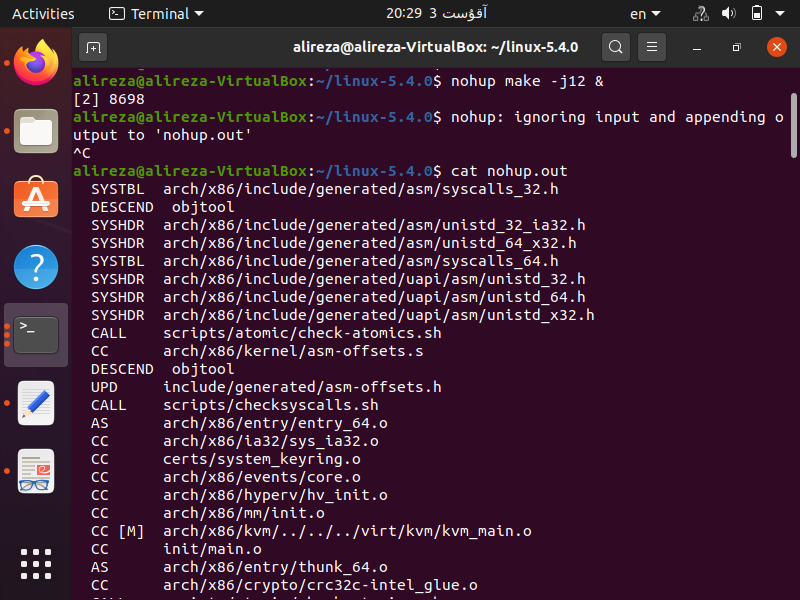
\includegraphics[scale=0.4]{img/pic11.png}
 			 \end{figure}
 		 
 		 \begin{figure}[!hpbt]
 		 	\centering
 		 	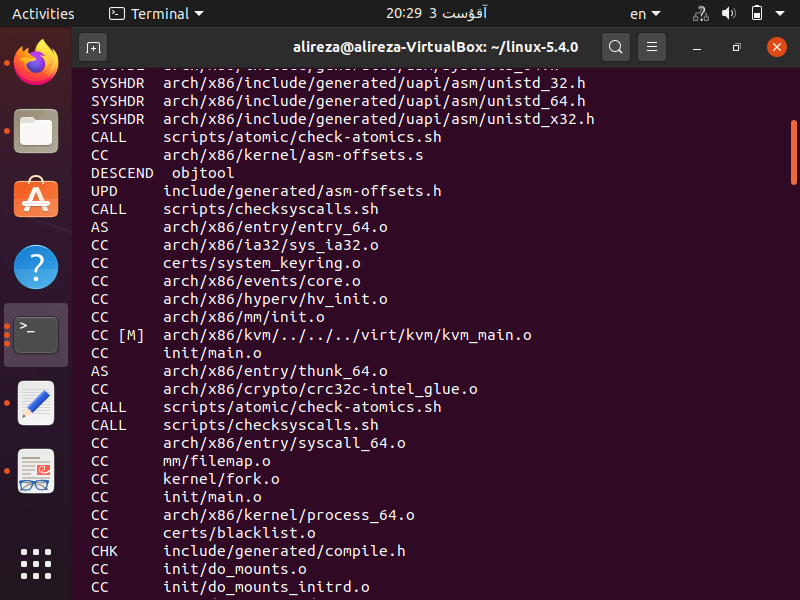
\includegraphics[scale=0.4]{img/pic12.png}
 		 	
 		 \end{figure}
 	  		 	\begin{figure}[!hpbt]
		 	 	\centering
		 	 	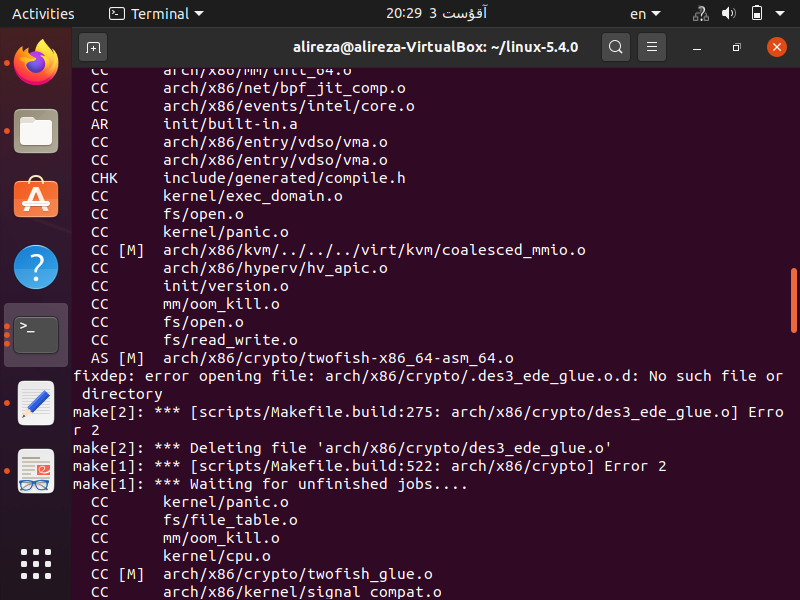
\includegraphics[scale=0.4]{img/pic13.png}
		 	 \end{figure}
	 	 \begin{figure}[!hpbt]
	 	 	\centering
	 	 	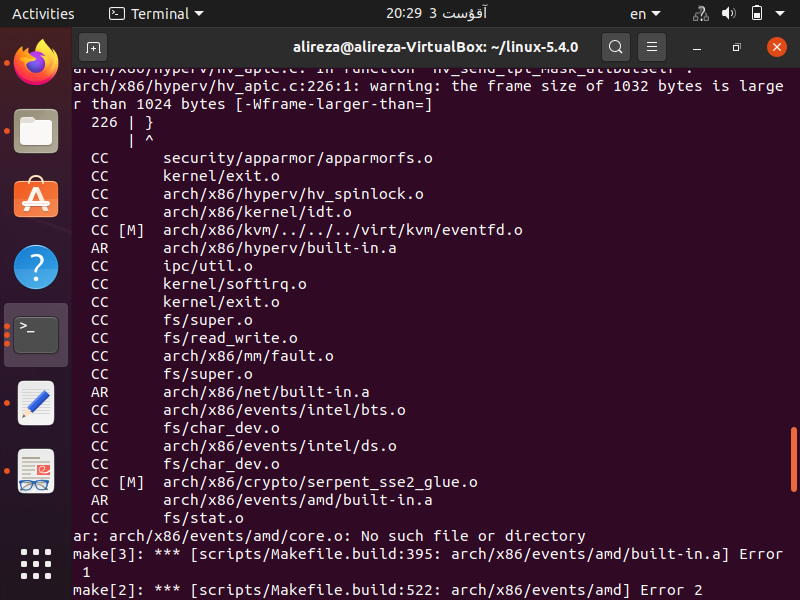
\includegraphics[scale=0.4]{img/pic14.png}
	 	 \end{figure}
 	 \begin{figure}[!hpbt]
 	 	\centering
 	 	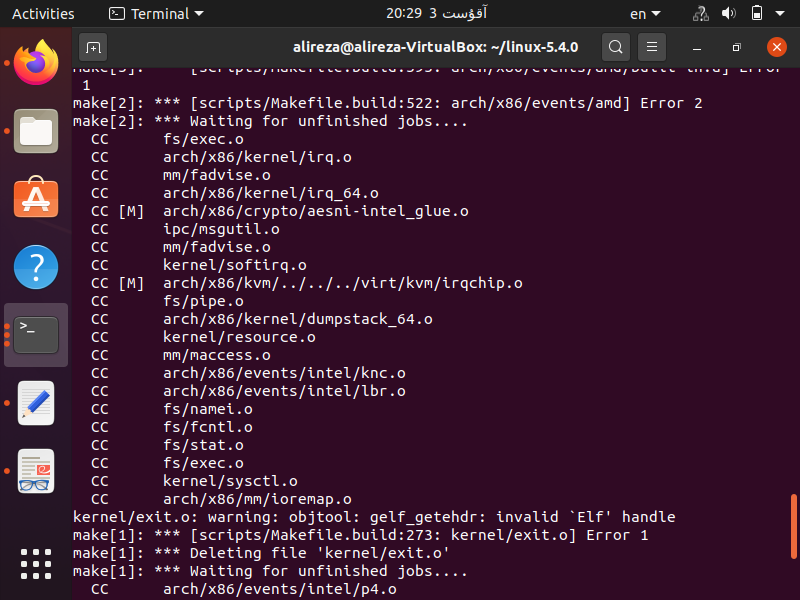
\includegraphics[scale=0.4]{img/pic15.png}
 	 \end{figure}
  			\begin{figure}[!hpbt]
  				\centering
  				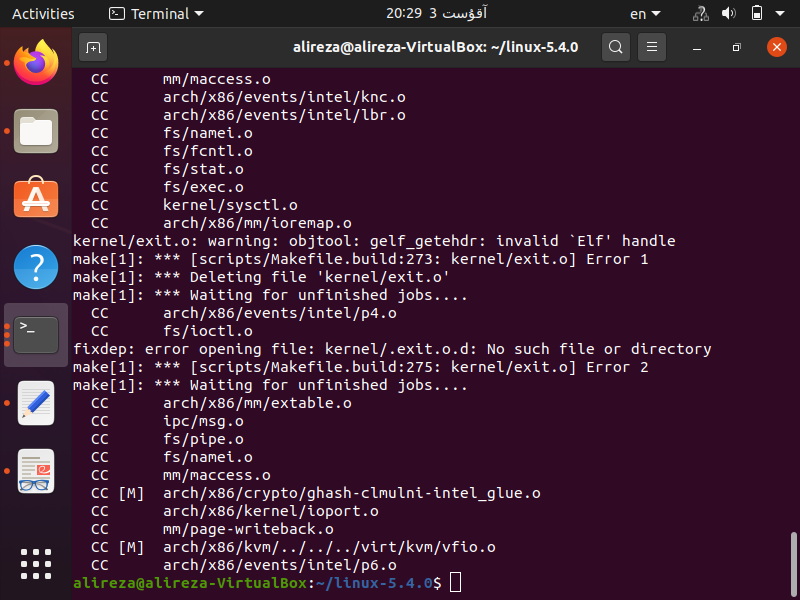
\includegraphics[scale=0.4]{img/pic16.png}
  			\end{figure}
 			 \item 
 			 
 			 با استفاده از فایل \lr{test.c} می‌خواهیم خروجی آن را ببینیم که با اجرای فایل خروجی \lr{test} حاصل از \lr{gcc test.c -o test} آن را بدست می‌آوریم.
 			 \begin{figure}[!hpbt]
 			 	\centering
 			 	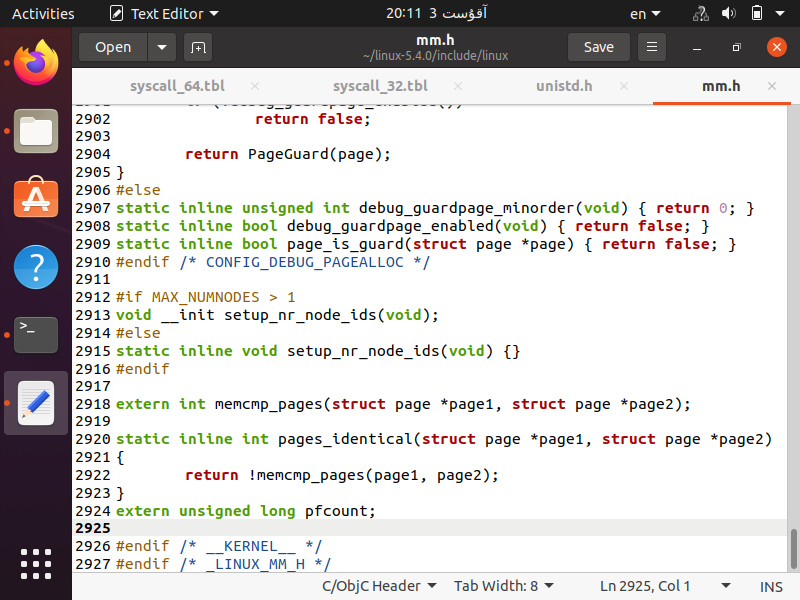
\includegraphics[scale=0.4]{img/pic4.png}
 			 \end{figure}
 			 \begin{figure}[!hpbt]
 			 	\centering
 			 	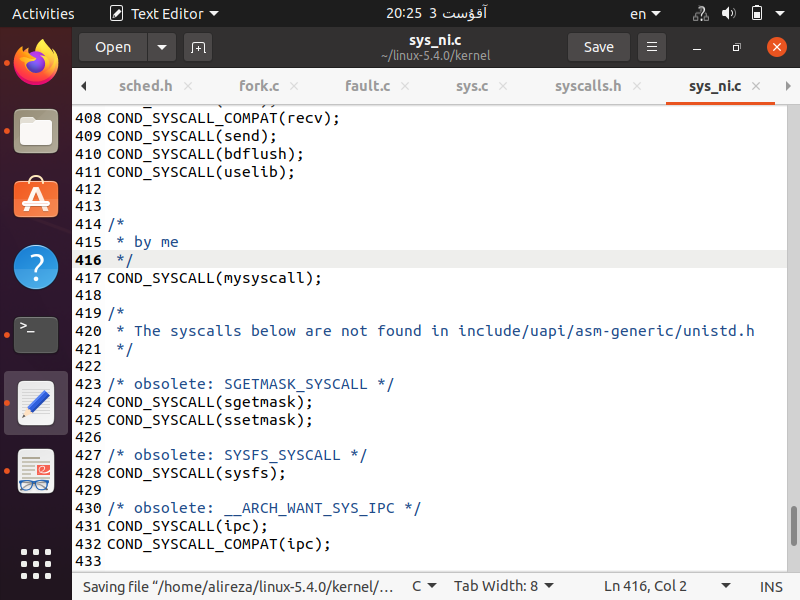
\includegraphics[scale=0.4]{img/pic10.png}
 			 \end{figure}
 		 \begin{figure}[!hpbt]
 		 	\centering
 		 	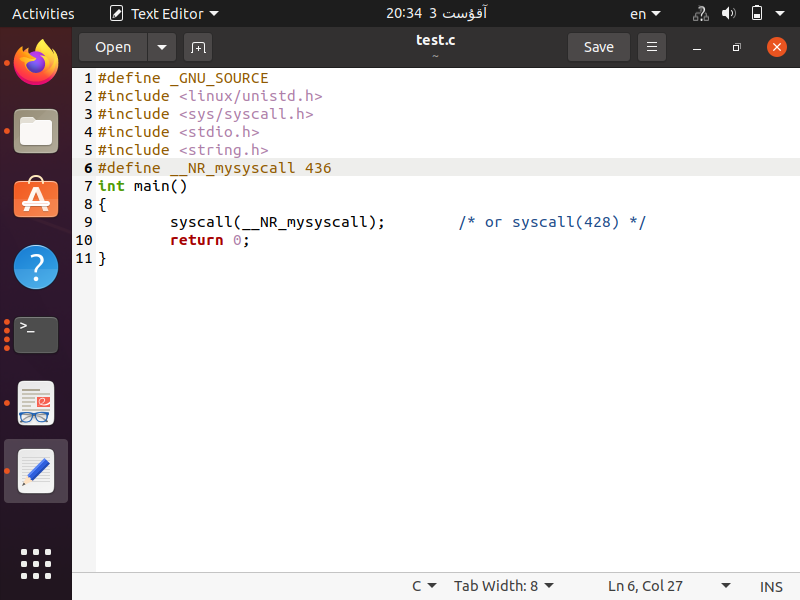
\includegraphics[scale=0.4]{img/pic17.png}
 		 \end{figure}
 	 
 			 \item 
 			 اگر خروجی را با \lr{dmesg} چک کنیم مشاهده می‌کنیم که به ترتیب مجموع تعداد \lr{page fault} ها و تعداد \lr{page fault} های حال حاضر را مشاهده کنیم.
		\end{enumerate}
	\end{itemize}